\section{Main Results}

\subsection{Primary Human Benchmark}

On the occurrence-matched fixed Human test set, tuned TissuePMHC reaches mean AUROC/AUPRC values of 0.8136/0.8126 across 77 tissue--HLA tasks. Accuracy is 0.7456, MCC is 0.4918, and the mean AUROC of the ten most difficult tasks is 0.6608 (Table~\ref{tab:human-standard}).

\begin{table*}[tbp]
\centering
\caption{Human architecture survey on the occurrence-matched fixed test, ordered by mean AUROC. The table asks which completed architecture has the strongest internal fixed-test task-macro performance; it does not establish universal architectural superiority. All systems use the same 77 tissue--HLA tasks. Values are arithmetic means $\pm$ sample standard deviations of the three seed-level task-macro metrics for seeds 20260704--20260706, except the $\dagger$ row-level prediction aggregate. Accuracy and MCC are means over seeds; Worst-10 is computed after first averaging each task over seeds. The tuned configuration was selected by training-only out-of-fold performance before the fixed test was opened.}
\label{tab:human-standard}
\scriptsize
\renewcommand{\arraystretch}{1.04}
\setlength{\tabcolsep}{2pt}
\begin{tabularx}{\textwidth}{>{\raggedright\arraybackslash}Xrrrrr}
\toprule
Model & AUROC & AUPRC & Acc. & MCC & Worst-10 \\
\midrule
Neural single-task MLP & 0.6908 $\pm$ 0.0061 & 0.6959 $\pm$ 0.0070 & 0.6389 & 0.2795 & 0.5670 \\
HLA pseudo-sequence conditioned & 0.7081 $\pm$ 0.0089 & 0.7136 $\pm$ 0.0071 & 0.6570 & 0.3184 & 0.5546 \\
Tissue-grouped hard sharing & 0.7114 $\pm$ 0.0054 & 0.7127 $\pm$ 0.0058 & 0.6555 & 0.3138 & 0.5828 \\
Conditioned tissue and HLA IDs & 0.7150 $\pm$ 0.0073 & 0.7191 $\pm$ 0.0052 & 0.6623 & 0.3281 & 0.5606 \\
HLA ID + pseudo-sequence hybrid & 0.7331 $\pm$ 0.0058 & 0.7359 $\pm$ 0.0055 & 0.6746 & 0.3530 & 0.5787 \\
FAMO shared heads & 0.7379 $\pm$ 0.0097 & 0.7410 $\pm$ 0.0105 & 0.6801 & 0.3620 & 0.5897 \\
HLA-grouped hard sharing & 0.7525 $\pm$ 0.0019 & 0.7517 $\pm$ 0.0012 & 0.6909 & 0.3843 & 0.6046 \\
Selective global/HLA grouping & 0.7643 $\pm$ 0.0015 & 0.7632 $\pm$ 0.0037 & 0.6994 & 0.4023 & 0.6143 \\
Validation-softmax ensemble & 0.7722 $\pm$ 0.0018 & 0.7729 $\pm$ 0.0035 & 0.7042 & 0.4118 & 0.6227 \\
MMoE, 6 experts $\times$ width 128 & 0.7727 $\pm$ 0.0010 & 0.7745 $\pm$ 0.0019 & 0.7074 & 0.4190 & 0.6176 \\
Shared encoder with task heads & 0.7758 $\pm$ 0.0087 & 0.7759 $\pm$ 0.0053 & 0.7052 & 0.4138 & 0.6337 \\
MMoE & 0.7763 $\pm$ 0.0046 & 0.7792 $\pm$ 0.0045 & 0.7063 & 0.4167 & 0.6275 \\
Validation-delta clipped ensemble & 0.7785 $\pm$ 0.0017 & 0.7799 $\pm$ 0.0037 & 0.7098 & 0.4227 & 0.6284 \\
MMoE, 4 experts $\times$ width 256 & 0.7816 $\pm$ 0.0023 & 0.7827 $\pm$ 0.0050 & 0.7146 & 0.4335 & 0.6357 \\
Fixed global/HLA dual-branch average & 0.7824 $\pm$ 0.0016 & 0.7851 $\pm$ 0.0035 & 0.7128 & 0.4287 & 0.6301 \\
Tissue/HLA auxiliary supervision & 0.7831 $\pm$ 0.0025 & 0.7840 $\pm$ 0.0003 & 0.7129 & 0.4315 & 0.6421 \\
Auxiliary-global + auxiliary-HLA dual branch & 0.7832 $\pm$ 0.0028 & 0.7836 $\pm$ 0.0026 & 0.7150 & 0.4342 & 0.6407 \\
DB-MTL shared heads & 0.7835 $\pm$ 0.0073 & 0.7800 $\pm$ 0.0101 & 0.7206 & 0.4436 & 0.6345 \\
Pair-ranking objective & 0.7841 $\pm$ 0.0030 & 0.7825 $\pm$ 0.0034 & 0.7187 & 0.4395 & 0.6431 \\
Auxiliary-global + plain-HLA dual branch & 0.7911 $\pm$ 0.0038 & 0.7916 $\pm$ 0.0054 & 0.7203 & 0.4447 & 0.6480 \\
MLP dual-branch rank average$^\dagger$ & 0.8033 & 0.8018 & 0.7326 & 0.4656 & 0.6559 \\
TissuePMHC (untuned) & 0.8082 $\pm$ 0.0033 & 0.8081 $\pm$ 0.0032 & 0.7368 & 0.4742 & 0.6604 \\
TissuePMHC (tuned) & \textbf{0.8136 $\pm$ 0.0021} & \textbf{0.8126 $\pm$ 0.0021} & \textbf{0.7456} & \textbf{0.4918} & \textbf{0.6608} \\
\bottomrule
\end{tabularx}
\end{table*}

Figure~\ref{fig:human-standard} visualizes the complete 23-method survey from Table~\ref{tab:human-standard} in the same AUROC order. Showing every surveyed architecture in one panel makes the separation between simple conditioning, hard sharing, adaptive sharing, dual-branch models, and the tuned TissuePMHC configuration directly visible without introducing a second comparison panel.

\begin{figure*}[t]
\centering
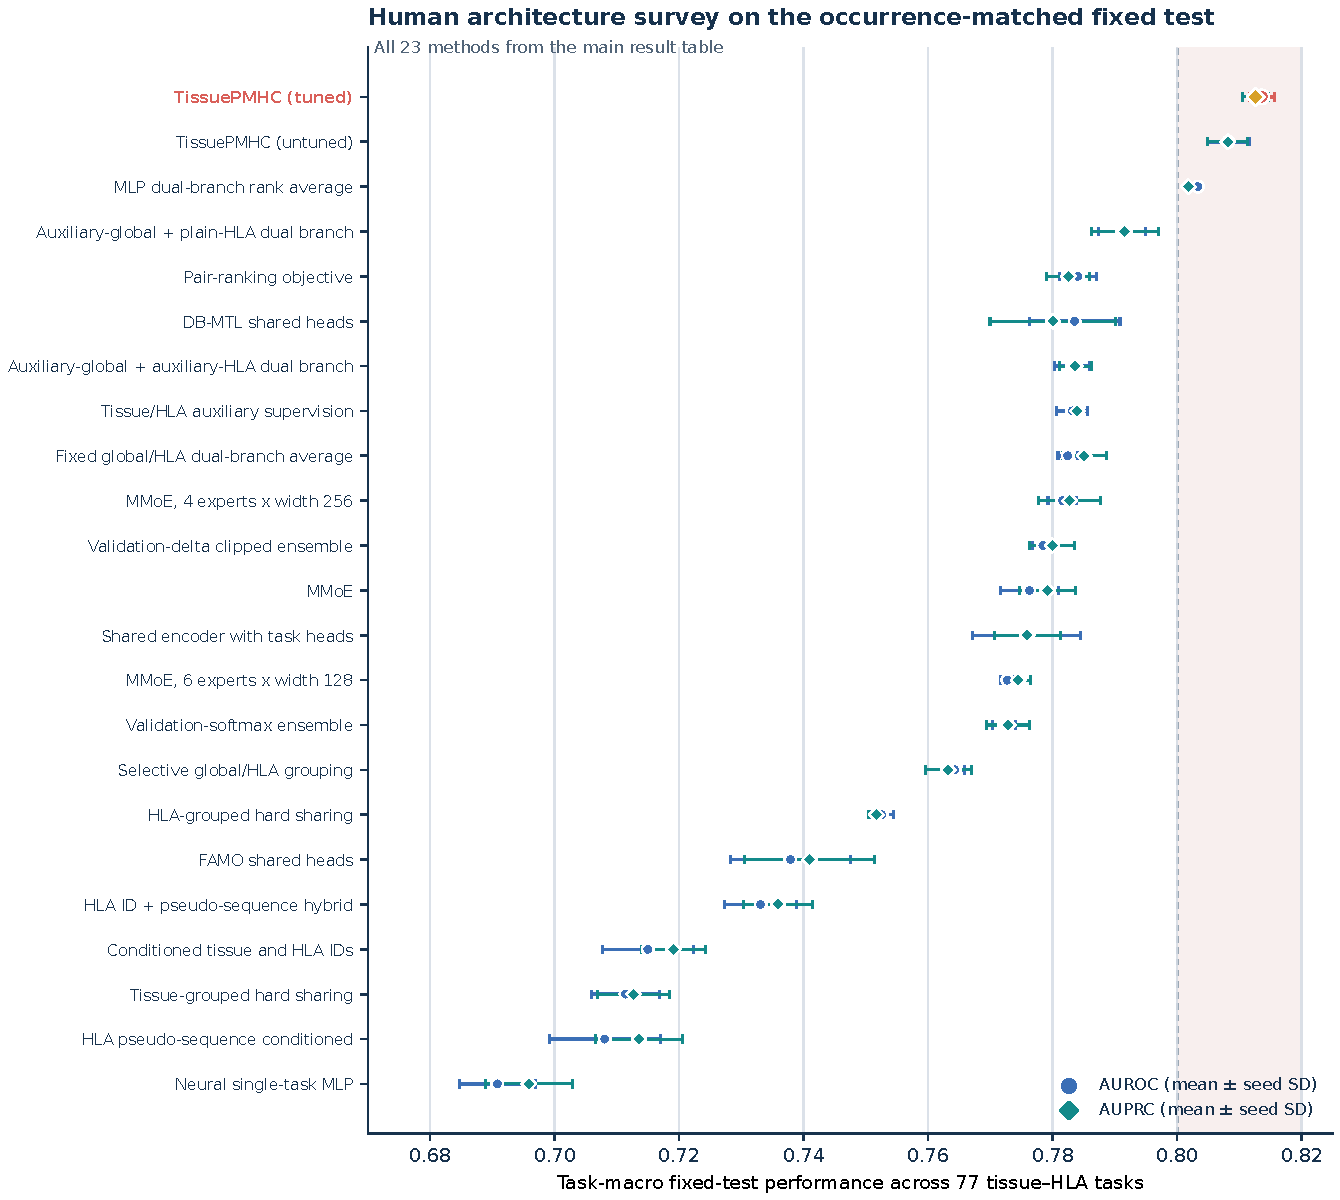
\includegraphics[width=0.88\textwidth]{figures/figure5_human_architecture_survey.pdf}
\caption{Human architecture survey on the occurrence-matched fixed test. All 23 methods and their ordering correspond to Table~\ref{tab:human-standard}. Circles show task-macro AUROC and diamonds show task-macro AUPRC across the same 77 tissue--HLA tasks; horizontal bars are sample standard deviations of the three seed-level macro metrics. The MLP dual-branch rank average is a row-level prediction aggregate and therefore has no seed-level interval. The shaded region begins at AUROC 0.8000, and the tuned TissuePMHC row is highlighted.}
\label{fig:human-standard}
\end{figure*}
\FloatBarrier

Relative to untuned TissuePMHC, training-only tuning increases Human mean AUROC by 0.0054 and mean AUPRC by 0.0045. The task-wise distribution of this change, together with the corresponding Mouse comparison and prespecified statistical summary, appears in Figure~\ref{fig:tuning-delta-by-species}.

\subsection{Replication on the Mouse Benchmark}

The Mouse benchmark applies the same pair definition, 50-pair-per-task test quota, and three seeds without transferring Human parameters. Table~\ref{tab:mouse-baselines} reports the completed fixed-test survey.

\begin{table*}[t]
\centering
\caption{Mouse occurrence-matched fixed-test survey across 11 tissue--H2 tasks, ordered by mean AUROC. The table asks the same within-species architecture question as Table~\ref{tab:human-standard}, using the same AUROC, AUPRC, accuracy, and MCC definitions; the completed model inventories differ and are not ranked across species. Values are arithmetic means $\pm$ sample standard deviations of three seed-level task-macro metrics; accuracy and MCC are means over seeds. Worst-5 is computed after first averaging each task over seeds and is not numerically interchangeable with Human Worst-10. The tuned TissuePMHC configuration was selected by three-fold cross-validation confined to the Mouse training split before fixed-test evaluation. The row marked $\dagger$ aggregates row-level predictions and therefore has no seed-level standard deviation.}
\label{tab:mouse-baselines}
\scriptsize
\renewcommand{\arraystretch}{1.06}
\setlength{\tabcolsep}{2.0pt}
\begin{tabularx}{\textwidth}{>{\raggedright\arraybackslash}Xrrrrr}
\toprule
Model & AUROC & AUPRC & Acc. & MCC & Worst-5 \\
\midrule
Neural single-task MLP & 0.6866 $\pm$ 0.0062 & 0.6960 $\pm$ 0.0039 & 0.6400 & 0.2826 & 0.6012 \\
Tissue-grouped hard sharing & 0.6941 $\pm$ 0.0106 & 0.6866 $\pm$ 0.0142 & 0.6491 & 0.3000 & 0.6160 \\
Conditioned tissue and H2 IDs & 0.6995 $\pm$ 0.0089 & 0.7051 $\pm$ 0.0122 & 0.6545 & 0.3123 & 0.6209 \\
H2 ID + pseudo-sequence hybrid & 0.7102 $\pm$ 0.0065 & 0.7180 $\pm$ 0.0197 & 0.6621 & 0.3280 & 0.6255 \\
H2 pseudo-sequence conditioned & 0.7254 $\pm$ 0.0109 & 0.7361 $\pm$ 0.0033 & 0.6685 & 0.3394 & 0.6447 \\
Selective global/H2 grouping & 0.7365 $\pm$ 0.0086 & 0.7418 $\pm$ 0.0067 & 0.6827 & 0.3682 & 0.6308 \\
Validation-softmax dual-branch ensemble & 0.7429 $\pm$ 0.0038 & 0.7492 $\pm$ 0.0068 & 0.6897 & 0.3822 & 0.6372 \\
Validation-delta clipped dual-branch ensemble & 0.7470 $\pm$ 0.0039 & 0.7529 $\pm$ 0.0063 & 0.6933 & 0.3892 & 0.6427 \\
Fixed global/H2 dual-branch average & 0.7505 $\pm$ 0.0035 & 0.7552 $\pm$ 0.0046 & 0.6973 & 0.3972 & 0.6512 \\
Shared encoder with task heads & 0.7513 $\pm$ 0.0151 & 0.7618 $\pm$ 0.0175 & 0.6921 & 0.3867 & 0.6624 \\
MMoE, 4 experts $\times$ width 256 & 0.7571 $\pm$ 0.0111 & 0.7668 $\pm$ 0.0190 & 0.6970 & 0.3963 & 0.6637 \\
Auxiliary-global + auxiliary-H2 dual branch & 0.7577 $\pm$ 0.0106 & 0.7648 $\pm$ 0.0122 & 0.6915 & 0.3858 & 0.6679 \\
MMoE, 6 experts $\times$ width 128 & 0.7609 $\pm$ 0.0184 & 0.7672 $\pm$ 0.0189 & 0.7021 & 0.4076 & 0.6802 \\
Auxiliary-global + plain-H2 dual branch & 0.7613 $\pm$ 0.0142 & 0.7679 $\pm$ 0.0180 & 0.7033 & 0.4097 & 0.6637 \\
CAGrad shared heads & 0.7674 $\pm$ 0.0176 & 0.7796 $\pm$ 0.0179 & 0.7000 & 0.4025 & 0.6762 \\
MLP dual-branch rank average$^\dagger$ & 0.7699 & 0.7793 & 0.7082 & 0.4166 & 0.6702 \\
TissuePMHC (untuned) & 0.7705 $\pm$ 0.0036 & 0.7785 $\pm$ 0.0031 & 0.7085 & 0.4174 & 0.6759 \\
Task-balanced shared heads & 0.7708 $\pm$ 0.0140 & 0.7835 $\pm$ 0.0155 & 0.7039 & 0.4102 & 0.6837 \\
DB-MTL shared heads & 0.7753 $\pm$ 0.0175 & 0.7880 $\pm$ 0.0179 & 0.7073 & 0.4169 & 0.6908 \\
TissuePMHC (tuned) & \textbf{0.8194 $\pm$ 0.0157} & \textbf{0.8279 $\pm$ 0.0121} & \textbf{0.7606} & \textbf{0.5216} & \textbf{0.7210} \\
\bottomrule
\end{tabularx}
\end{table*}
\FloatBarrier

Tuned TissuePMHC has the largest surveyed Mouse mean AUROC and AUPRC, reaching 0.8194/0.8279; its accuracy and MCC are 0.7606 and 0.5216. Its seed-level variation overlaps less strongly with the previous leading DB-MTL mean than the untuned model did, but this remains a comparison on one internal fixed test rather than evidence of universal architectural superiority.

\subsection{Cross-species Synthesis}

After matching MHC restriction, parent protein, and total positive tissue-occurrence count, sequence-based models retain above-random discrimination in both species. Tuned TissuePMHC reaches mean AUROC/AUPRC values of 0.8136/0.8126 in Human and 0.8194/0.8279 in Mouse. In both species, the occurrence-count-only score is exactly 0.5000 in every task. The remaining signal is therefore not explained by the controlled occurrence-count shortcut, although it can still reflect antigen processing, protein abundance, cell composition, or study structure.
